% Encoding: UTF-8
%%%%%%%%%%%%%%%%%%%%%%%%%%%%%%%%%%%%%%%%%%%%%%%%%%%%%%%%%%%%%%%%%%%%%%%%%%%%%%%

\documentclass[xcolor=pdftex,dvipsnames,table]{beamer}
\setbeamertemplate{navigation symbols}{}%remove navigation symbols
%%%%%%%%%%%%%%%%%%%%%%%%%%%%%%%%%%%%%%%%%%%%%%%%%%%%%%%%%%%%%%%%%%%%%%%%%%%%%%%

% Language settings
% IMPORTANT: If you change the language settings, make sure to run
% cleantex prior to any latex/pdflatex to remove all .aux files, else
% latex might fail!
\usepackage[english]{babel}
%\usepackage[german]{babel}

%\usepackage{graphicx}
\usepackage[utf8]{inputenc}
%\usepackage{mathptmx}
\usepackage{setspace}
\usepackage{color}
\usepackage{listings}
\usepackage{svg}
\usepackage{amsmath}

%%%%%%%%%%%%%%%%%%%%%%%%%%%%%%%%%%%%%%%%%%%%%%%%%%%%%%%%%%%%%%%%%%%%%%%%%%%%%%%

% IMPORTANT/TODO: currently only PDF graphic files should be used, PNG
% or JPEG may harm the Adobe Reader colour palette and result in
% strange display colours.
%\DeclareGraphicsExtensions{.pdf}
%\outputdirectory{{./pdfs/}}
\graphicspath{{./img/}}

%%%%%%%%%%%%%%%%%%%%%%%%%%%%%%%%%%%%%%%%%%%%%%%%%%%%%%%%%%%%%%%%%%%%%%%%%%%%%%%
%% Presentation main settings
%%%%%%%%%%%%%%%%%%%%%%%%%%%%%%%%%%%%%%%%%%%%%%%%%%%%%%%%%%%%%%%%%%%%%%%%%%%%%%%

\title{Systemnahe Informatik}
\subtitle{Übungsgruppe Xeon Phi}
\author{Dominik Walter}
\date{Sommersemester 2018}


%%%%%%%%%%%%%%%%%%%%%%%%%%%%%%%%%%%%%%%%%%%%%%%%%%%%%%%%%%%%%%%%%%

\begin{document}

\section*{Titlepage}
\begin{frame}
  \frametitle{\ }
  \titlepage
\end{frame}

%%%%%%%%%%%%%%%%%%%%%%%%%%%%%%%%%%%%%%%%%%%%%%%%%%%%%%%%%%%%%%%%%%%%%%%%%%%%%%%

\begin{frame}[fragile]
	\frametitle{Cache-Effizienz}
		\begin{lstlisting}
void work(char* buf, int size, int n) {
	srand(time(0));
	int index;
	for (int i = 0; i < n; i++) {
		index = rand() % size;
		buf[index] = buf[index] * 2;
	}
}
		\end{lstlisting}
\end{frame}

\begin{frame}
	\frametitle{Cache-Effizienz}

	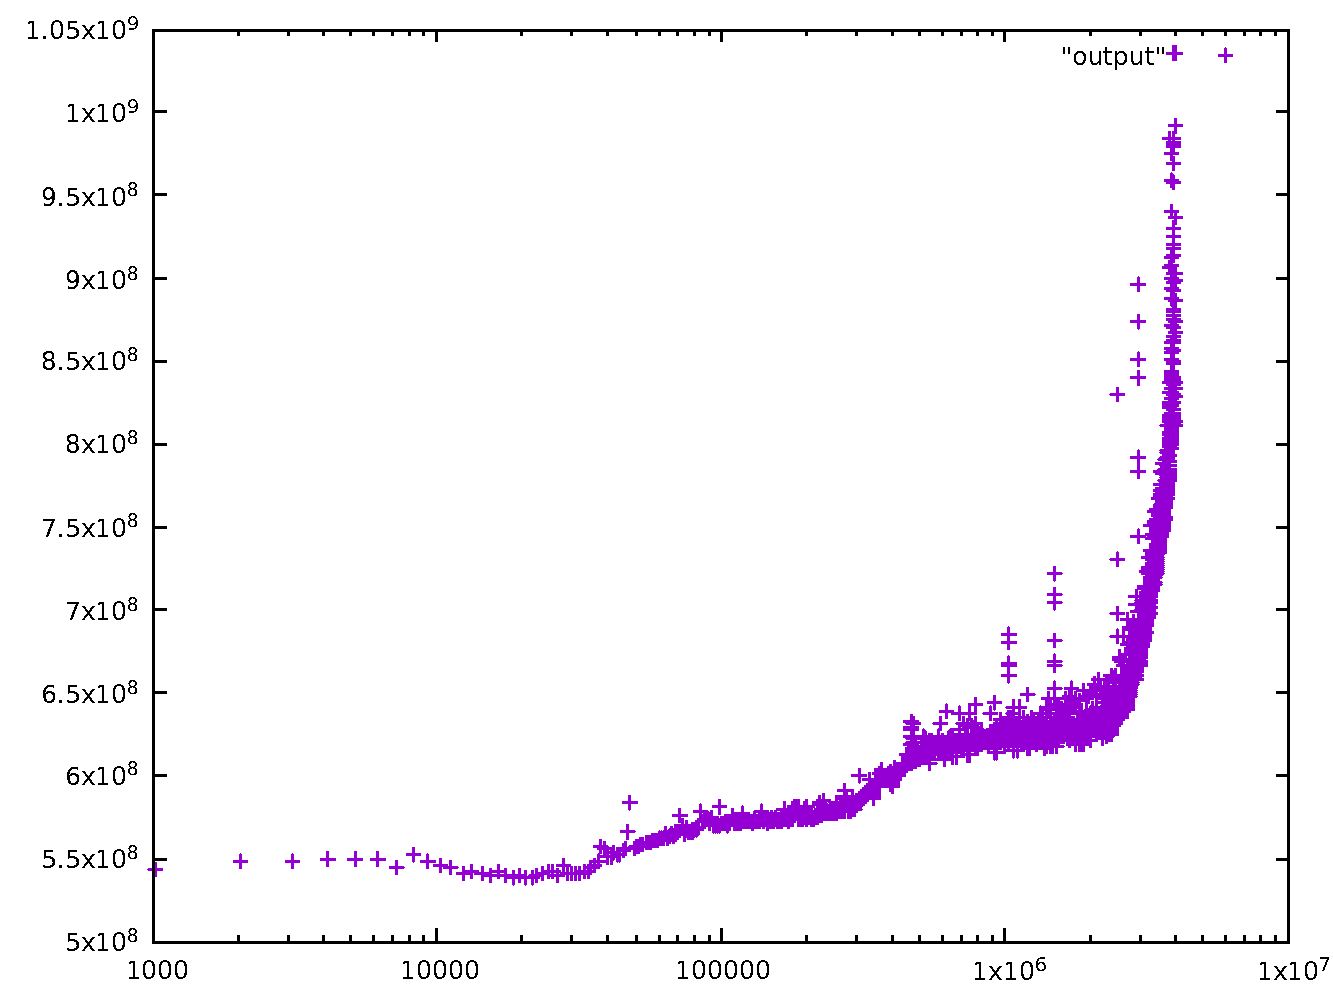
\includegraphics[width=10cm]{cache.pdf}
\end{frame}

\end{document}

%%%%%%%%%%%%%%%%%%%%%%%%%%%%%%%%%%%%%%%%%%%%%%%%%%%%%%%%%%%%%%%%%%%%%%%%%%%%%%%
